\documentclass[tikz,border=12pt]{standalone}
\usepackage{tikz}
\usetikzlibrary{shapes.geometric,arrows.meta,positioning,fit,backgrounds,calc}

\renewcommand{\familydefault}{\sfdefault}
\definecolor{cborder}{HTML}{1E293B}
\definecolor{cbg}{HTML}{F8FAFC}
\definecolor{cbox}{HTML}{FFFFFF}
\definecolor{cblue}{HTML}{1E40AF}
\definecolor{cbluelight}{HTML}{EFF6FF}
\definecolor{cgray}{HTML}{64748B}
\definecolor{camber}{HTML}{D97706}
\definecolor{camberlight}{HTML}{FFFBEB}

\begin{document}
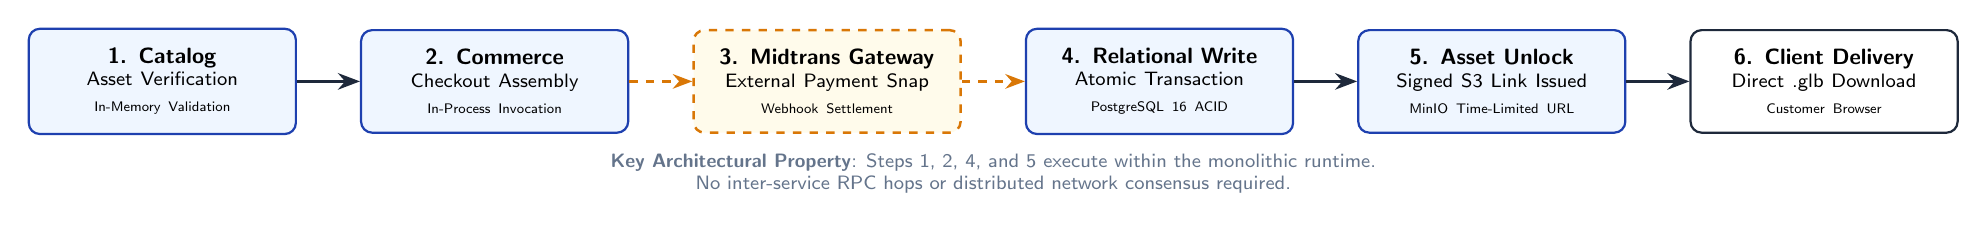
\begin{tikzpicture}[
    font=\small,
    >=Stealth,
    node distance=0.8cm and 0.8cm,
    stepbox/.style={
        draw=cborder,
        fill=cbox,
        rounded corners=4pt,
        line width=0.8pt,
        align=center,
        inner sep=7pt,
        font=\footnotesize,
        text width=2.9cm,
        minimum height=1.3cm
    },
    monostep/.style={
        draw=cblue,
        fill=cbluelight,
        rounded corners=4pt,
        line width=0.8pt,
        align=center,
        inner sep=7pt,
        font=\footnotesize,
        text width=2.9cm,
        minimum height=1.3cm
    },
    extstep/.style={
        draw=camber,
        fill=camberlight,
        dashed,
        rounded corners=4pt,
        line width=0.9pt,
        align=center,
        inner sep=7pt,
        font=\footnotesize,
        text width=2.9cm,
        minimum height=1.3cm
    },
    flow/.style={
        ->,
        line width=1.1pt,
        draw=cborder
    },
    extflow/.style={
        ->,
        line width=0.9pt,
        draw=camber,
        dashed
    }
]

    % Step 1: Catalog
    \node[monostep] (s1) {
        \textbf{1. Catalog}\\
        \scriptsize Asset Verification\\
        \tiny In-Memory Validation
    };

    % Step 2: Commerce
    \node[monostep, right=0.8cm of s1] (s2) {
        \textbf{2. Commerce}\\
        \scriptsize Checkout Assembly\\
        \tiny In-Process Invocation
    };

    % Step 3: Payment Gateway (External)
    \node[extstep, right=0.8cm of s2] (s3) {
        \textbf{3. Midtrans Gateway}\\
        \scriptsize External Payment Snap\\
        \tiny Webhook Settlement
    };

    % Step 4: DB Write
    \node[monostep, right=0.8cm of s3] (s4) {
        \textbf{4. Relational Write}\\
        \scriptsize Atomic Transaction\\
        \tiny PostgreSQL 16 ACID
    };

    % Step 5: MinIO S3 URL
    \node[monostep, right=0.8cm of s4] (s5) {
        \textbf{5. Asset Unlock}\\
        \scriptsize Signed S3 Link Issued\\
        \tiny MinIO Time-Limited URL
    };

    % Step 6: Client Delivery
    \node[stepbox, right=0.8cm of s5] (s6) {
        \textbf{6. Client Delivery}\\
        \scriptsize Direct .glb Download\\
        \tiny Customer Browser
    };

    % Arrows
    \draw[flow] (s1) -- (s2);
    \draw[extflow] (s2) -- (s3);
    \draw[extflow] (s3) -- (s4);
    \draw[flow] (s4) -- (s5);
    \draw[flow] (s5) -- (s6);

    % Legend / Invariant annotation at bottom
    \node[below=0.8cm of $(s3)!0.5!(s4)$, font=\scriptsize, align=center, text=cgray] {
        \textbf{Key Architectural Property}: Steps 1, 2, 4, and 5 execute within the monolithic runtime.\\
        No inter-service RPC hops or distributed network consensus required.
    };

\end{tikzpicture}
\end{document}
